\chapter{The Sabbath God vs. Sunday God - J. B. Frisbie}

There are other articles written on the \emcap{personality of God} by our pioneers and it would be too much to include everything here, but we would like to add one more testimony from brother J. B. Frisbie’s article where he compares the Sabbath God with the Sunday God. He compares the truth on the \emcap{personality of God} expressed in the first point of the \emcap{Fundamental Principles} with the Trinity doctrine. Let us take a look at a portion of his article, “\textit{The Seventh Day-Sabbath Not Abolished}” from the Review and Herald, March 7, 1854.

\begin{figure}[hp]
    \centering
    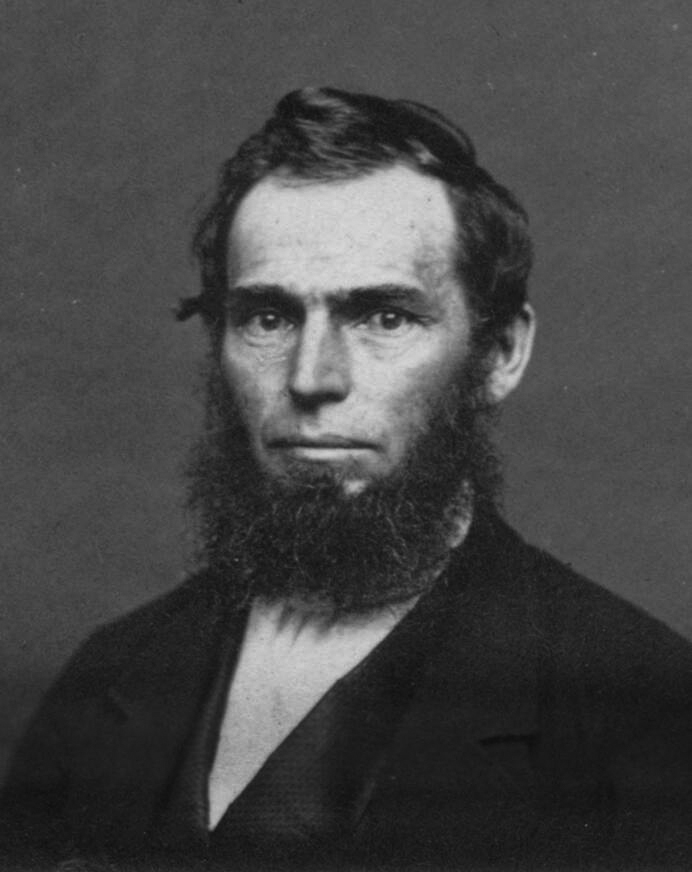
\includegraphics[width=1\linewidth]{images/j-b-frisbie.jpg}
    \caption*{John Byington Frisbie (1816-1882)}
    \label{fig:j-b-frisbie}
\end{figure}

\section*{The Sabbath God}

\others{After we know and remember God, by keeping his holy Sabbath, \textbf{then the Bible will teach of his personality and dwelling place}. \textbf{Man is in the image and likeness of God}. Genesis 1:26. ‘And God said, Let us (speaking to his son) make man in our image, after our likeness’. Chap 2:7. ‘And the Lord God formed man of the dust of the ground, and breathed into his nostrils the breath of life: and man became a living soul’. Genesis 9:6; 1 Corinthians 11:7; James 3:9. \textbf{That which was made in \underline{the image and likeness of God} was made of the dust of the ground called man}.}

\othersnogap{This is known to be the true sense from other testimonies that may be given from the Bible. \textbf{Jesus was in the form of a man and the express image of his Father’s person}.}

\othersnogap{Philippians 2:6-8. \textbf{Christ Jesus}: ‘Who, being in \textbf{the form of God}, thought it not robbery to be \textbf{equal with God}. But made himself of no reputation, and took upon him \textbf{the form of a servant}, and was \textbf{made in the likeness of men’}. 2 Corinthians 4:4. \textbf{‘And being formed in fashion as a man’}, etc. Colossians 1:15. ‘\textbf{Who is the image of the invisible God}’.}

\othersnogap{Hebrews 1:3. \textbf{The Son; ‘Who being the brightness of his glory, and the express image of his person’}. In this sense could Jesus say to Philip in truth, ‘He that hath seen me hath seen the Father.’ John 14:9. Some seem to suppose it argues \textbf{against the personality of God, \underline{because he is a Spirit, and say that he is without body, or parts}}. John 4:24. ‘\textbf{God is a Spirit}’. Hebrews 1:7. ‘\textbf{Who maketh his angels spirits}’. \textbf{Who would pretend to say that angels have no bodies or parts because they are spirits}. \textbf{\underline{None the less is God a spiritual being having body and parts as we may learn by his having a dwelling place and because he has and may be seen}}. Exodus 33:23. ‘And I will take away mine hand, and thou shalt\textbf{ see my back parts}, but my \textbf{face shall not be seen}’. Matthew 5:8. ‘Blessed are the pure in heart, for \textbf{they shall see God}’. Hebrews 12:14. ‘Follow peace with all men, and holiness, without which \textbf{no man shall see the Lord}’. Matthew 18:10. ‘That in heaven their angels do \textbf{always behold the face of my Father which is in heaven}’. Matthew 6:9. ‘After this manner therefore pray ye, \textbf{Our Father which art in heaven}’, etc. John 6:38. ‘For I \textbf{came down from heaven} not to do mine own will, but the will of him that sent me’. Chap 16:28. ‘\textbf{I came forth from the Father, and am come into the world}: again I \textbf{leave the world, and go to the Father}’.}

\othersnogap{\textbf{Does not God say he fills immensity of space? \underline{We answer, No}}. Psalm 139:7, 8. ‘Whither shall I go \textbf{from thy Spirit}? or whither shall I flee \textbf{from thy presence}? If I ascend up into heaven, thou art there’, etc. \textbf{\underline{God by his Spirit may fill heaven and earth}}, etc. \textbf{Some confound God with his Spirit, which makes confusion}. Psalm 11:4. ‘\textbf{The Lord is in his holy temple, the Lord’s throne is in heaven}: his eyes behold’, etc. Habakkuk 2:20; Psalm 102:19. ‘For he hath looked \textbf{down from the height of his Sanctuary}; \textbf{\underline{from heaven} did the Lord behold the earth’}. 1 Peter 3:12. ‘For the eyes of the Lord are over the righteous, and his ears are open unto their prayers’, etc. Psalm 80:1. ‘Give ear, O Shepherd of Israel, thou that leadest Joseph like a flock; thou \textbf{that dwellest between the cherubims}, shine forth’. Psalm 99:1; Isaiah 37:16.}

\othersnogap{John 14:2. ‘In my Father’s house are many mansions. I go to prepare a place for you’. Revelation 21:2-5; Hebrews 11:6. ‘For he that cometh to God must believe that he is’, etc. \textbf{This testimony we deem highly important at this time, to know that there is a God. We have no doubt that if our eyes could be opened in vision, or see as angels see, we should see God in heaven sitting on his throne, and is present to all that exists, however distant from him in his creation}.}[\href{https://documents.adventistarchives.org/Periodicals/RH/RH18540307-V05-07.pdf}{Adventist Review and Sabbath Herald, March 7, 1854}, J. B. Frisbie, “The Seventh-Day Sabbath Not Abolished”, p. 50]

Here we see the same argument and reasoning, that God is a personal spiritual Being. This God is the Sabbath God. Brother Frisbie compares this God with the Sunday God, who is a trinitarian God.

\section*{The Sunday God}

\others{We will make a few extracts, that the reader may \textbf{see the broad contrast between \underline{the God of the Bible} brought to light through Sabbath-keeping, and the god in the dark through Sunday-keeping}. Catholic Catechism Abridged by the Rt. Rev. John Dubois, Bishop of New York. Page 5. ‘\textbf{Ques. Where is God? Ans. God is everywhere}. Q. Does God see and know all things? A. Yes, he does know and see all things. \textbf{Q. Has God any body? A. \underline{No; God has no body, he is a pure Spirit}}. \textbf{Q. Are there more Gods than one? A. No; there is but one God. Q. Are there more persons than one in God? A. \underline{Yes; in God there are three persons}. Q. Which are they? A. God the Father, God the Son and God the Holy Ghost. Q. Are there not three Gods? A. No; the Father, the Son and the Holy Ghost, are all but one and the same God}’.}

\othersnogap{The first article of the Methodist Religion, p. 8. \textbf{‘There is but one living and true God}, everlasting, \textbf{without body or parts}, of infinite power, wisdom and goodness: the maker and preserver of all things, visible and invisible. \textbf{And in unity of this God-head, there are three persons of one substance, power and eternity; the Father, the Son, and the Holy Ghost}.’}

\othersnogap{In this article like the Catholic doctrine, \textbf{we are taught that there are three persons of one substance,} power and eternity making\textbf{ in all one living and true God}, everlasting \textbf{without body or parts}. But in all this we are not told \textbf{what became of the body of Jesus who had a body when he ascended, who went to God who ‘is everywhere’ or nowhere}. Doxology.}

\othersnogap{‘\textbf{To God the Father, God the Son,}} \\
\others{\textbf{God the Spirit, three in one.}’} \\
\others{Again} \\
\others{‘Warms in the sun, refreshes in the breeze,} \\
\others{Glows in the stars, and blossoms in the trees.} \\
\others{\textbf{Lives through all life, extends through all extent},} \\
\others{Spreads undivided and operates unspent.’ - Pope.}

\othersnogap{These ideas well accord with those heathen philosophers. One says, ‘That water was the principle of all things, and that God is that intelligence, by whom all things are formed out of water.’ Another, ‘That air is God, that it is produced, that it is immense and infinite,’ etc. A third, ‘That God is a soul diffused throughout all beings of nature,’ etc. \textbf{Some, who had the idea of \underline{a pure Spirit}}. Last of all, ‘That God is an eternal substance.’}

\othersnogap{These extracts are taken from Rollin’s History, Vol. II, pp. 597-8, published by Harpers. \textbf{We should rather mistrust that the Sunday god came from the same source that Sunday-keeping did}. ‘Sunday was a name given by the heathens to the first day of the week, because it was the day on which they worshiped the sun.’ - Union Bible Dictionary. \textbf{Afterward modified by the Roman Catholic Church, in the form we now find it taught through the land}.}

\othersnogap{It is very natural to suppose when \textbf{the Pope set himself up to be God in the temple of God}, [2 Thessalonians 2:4] that he should have a day sanctified to his worship. This he has done. - Douay Catechism, p. 59. ‘Q. What is the best means to sanctify Sunday? A. By hearing mass, etc. This saying mass is for the priest to gabble over Latin, drink some wine, and give the people a wafer to eat.’}”“\others{But God sanctified his day because he had rested on it. Another day for a very different purpose. Genesis 2:3.}

\othersnogap{In days before the moral fall of Babylon God directed the minds of his honest children right in their prayers, whatever they might think at other times, but now since the apostasy the mind reaches to no god but to the people only, there are many prayers to men we know by their effect and eloquence. \textbf{We are truly thankful to our heavenly Father that \underline{he has led our minds from such folly}, to know, and remember \underline{his holy name} by keeping his holy day that we might love, serve and worthily \underline{glorify him through our great High Priest in the heavenly Sanctuary in this day of atonement}}.}[Ibid.][https://documents.adventistarchives.org/Periodicals/RH/RH18540307-V05-07.pdf]

Before becoming a Seventh-day Adventist, Frisbie was a Methodist preacher and a bitter opponent of Adventist beliefs. In 1853, after a debate on the Sabbath with Joseph Bates, he reversed his position and began to keep the Sabbath and preach the Seventh-day Adventist doctrine. He renounced Sunday, the Trinity, and accepted the Seventh-day Sabbath and the truth about God, that the Seventh-day Adventist’s taught in the first point of the \emcap{Fundamental Principles}.

Do other Adventist pioneers see discordance between the Trinity doctrine and the \emcap{personality of God} expressed in the first point of the \emcap{Fundamental Principles}?

% The Sabbath God vs. Sunday God - J. B. Frisbie

\begin{titledpoem}
    \stanza{
        On seventh day or first we kneel, \\
        But deeper truths these days reveal. \\
        Not just when we choose to pray, \\
        But which God we serve each day.
    }

    \stanza{
        The Sabbath God, a Being clear, \\
        With form and place, both far and near. \\
        In His image we were made, \\
        His Son the perfect likeness displayed. \\
    }

    \stanza{
        The Son, the Father's image bright, \\
        Shows us the path to truth and light. \\
        "Who's seen me has seen the Father too," \\
        Christ's words both powerful and true.
    }

    \stanza{
        The Sunday God, a trinity, \\
        Three persons in strange unity. \\
        Without body, without part, \\
        A concept born from human art.
    }

    \stanza{
        One God with face and hands and form, \\
        Who rested when creation's storm \\
        Had ceased its work on seventh day, \\
        This God commands we rest and pray.
    }

    \stanza{
        Not some essence spreading wide, \\
        Formless spirit with no side. \\
        But a Person on a throne, \\
        With His Son, yet not alone.
    }

    \stanza{
        So choose not merely when to kneel, \\
        But which God your heart finds real. \\
        The day we keep reveals our view \\
        Of which God we believe is true.
    }
\end{titledpoem}